\section{Abstract}

The project for Controls will involve controlling a doubly inverted pendulum with a linear ``cart''. The goals
of this project are to
\begin{enumerate}
\item Linearize the system about the stability point and design a controller for it.
\item Determine the limits of the controller with respect to each state variable(in isolation) 
\end{enumerate}

In order to simplify the model, the mass of the pendulums will be assumed to be at the end of the rod, rather
than in the middle as it would be for a constant density rod.

\begin{figure}[h]
  \centering
  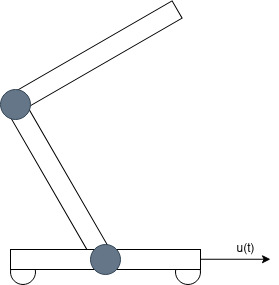
\includegraphics[width=0.25\textwidth]{../resources/doublyInvertedPendulum.jpg}
  \caption{System to be modeled}
  \label{}
\end{figure}
